\documentclass[../main]{subfiles}

\begin{document}

\section{Konventionen und Notation}

NOTATION ERKLAEREN (Vektor, Matrix, etc.)
\par\bigskip
Falls ein (Zeilen- oder Spalten-)Vektor $\vec{v}$ als Argument in eine Funktion $f$ gegeben wird, ist zu verstehen,
dass die einzelnen Komponenten des Vektors die Parameter der Funktion sind.
$f(\vec{v})=f(v_1,\cdots,v_n)$

\section{Machinelles Lernen - die Theorie}

Der Themenbereich des \textbf{Machinellen Lernens} beschäftigt sich mit Algorithmen und mathematischen Modellen, welche von selber lernen, Probleme zu loesen.
Hierzu werden keine expliziten Instruktionen fest einprogrammiert (engl.: hard coding), sondern das Modell wird trainiert und optimiert sich von selbst.
Dabei wird das Modell mit Trainingsdaten befuettern, mithilfe dessen eine Korrelation zwischen den Inputdaten und den Outputdaten erlernt werden soll.
Der Zusammenhang der Daten wird von den Modellen verallgemeinert und das Modell kann dann Vorhersagen fuer neue Daten machen. 

\subsection{Allgemeine Begriffe}

\subsubsection{Daten}

Der \textbf{Trainingsdatensatz} beinhaltet gewisse \textbf{Attribute}, die Merkmalstypen der Inputdaten.
Die \textbf{Features} sind dann die spezifischen Werte der Attribute eines Trainingssample.
Die sogenannten \textbf{Labels} sind die erwarteten Outputs, welche der Algorithmus vorherzusagen hat.
Diese Vorhersagen werden mit den Labels abgeglichen und so bewertet.
Anhand der Bewertungen wird dann eine Optimierung des Modells vorgenommen.
Unter korrekten Bedingungen (keine Ueberanpassung) findet kein Auswendiglernen der Trainingsdaten statt,
sondern ein Generalisieren des Zusammenhangs, anhand von Mustern und Gesetzmassigkeiten.
\par\medskip
Um eine Endgueltige Bewertung des Modells durchzufuehren, wird ein Testdatensatz, welcher nicht Teil des Trainingsdatensatz ist, genutzt um Vorhersagen zu machen.
Dies garantiert, dass kein Auswendiglernen moeglich ist.
\par\medskip
Die Inputs/Features werden in einem Vektor $\vec{x}=(x_1,x_2,...,x_n)^T$ und die Outputs/Vohersagen in einem Vektor $\vec{y}=(y_1,y_2,...,y_m)^T$ zusammengefasst.
Das gleiche macht man mit den Labels, wobei diese mit $\vec{\hat{y}}=(\hat{y}_1,\hat{y_2},...,\hat{y}_m)^T$ bezeichnet werden.
\par \medskip
Am Beispiel eines Datensatz, welcher fuer Bilderkennung von Hunden und Katzen genutzt wird, werden diese Begriffe verdeutlicht.
Die Inputdaten sind die Fotos von Hunden und Katzen. Deren Attribute sind die moeglichen RGB-Farbenwerte (drei Zahlen, welche von 0 bis 255 reichen) aller Pixel.
Die Features sind die spezifischen RGB-Werte aller Pixel. Die Outputdaten sind die Labels, welche in diesem Fall angeben, ob ein Hund oder eine Katze auf dem Bild gezeigt wird.
Dies wird meistens mit einer One-Hot-Kodierung bzw. einem One-Hot-Vektor gemacht. Jeder Labelart wird eine eigene Vektorkomponente zugewiesen. Falls das Label aktiv ist, ist die Komponent 1 ansonsten 0. Also Hund koennte als $\vec{l}_H=(1,0)^T$ reprasentiert werden und Katze als $\vec{l}_K=(0,1)^T$.

\begin{figure}[h!]
    \centering
    \begin{tikzpicture}[node distance=5cm,auto]
        
    \end{tikzpicture}
    
    \caption{eine Veranschaulichung eines Machine Learning Modells}
\end{figure}

\subsubsection{Modelle}
Ein \textbf{Modell} ist eine mathematische Funktion $\mathit{f}\colon \mathbb{R}^n \to \mathbb{R}^m$ welche die Inputs auf die Outputs abbildet $\vec{y}=\mathit{f}(\vec{x})$.
Im Zusammenhang mit Wertevorhersagen spricht man von einem Regressionsmodell.
Das Verhalten dieses Modells wird bestimmt durch seine \textbf{Modellparameter} $\phi_1, \phi_2, ...$.
Das Ziel ist es die Modellparameter so einzustellen, dass die Vorherrsagen $\vec{y}$ besser mit den Labels $\vec{\hat{y}}$ uebereinstimmen.
Dies wird iterativ gemacht, indem immer wieder leichte Anpassungen an den Parametern vorgenommen werden, bis sie das gewunschte Resultat liefern. 
\par\medskip
Das wohl einfachste Regressionsmodell ist eine Regressionsgerade. Diese ist angemessen, falls ein einfacher linearen Zusammenhang zwischen den Features und den Labels besteht.
$y=\phi_1x + \phi_0$. Nun muessten nur noch $\phi_0$ und $\phi_1$ bestimmt werden. 

Neben den gelernten Parametern, gibt es auch noch sogenannte \textbf{Hyperparameter}.
Diese koennen nicht erlernt werden, sondern muessen manuell vor dem Training gewaehlt werden und koennen den Lernvorgang erheblich beeinflussen.
\par\medskip
Fuer Machine Learning haben sich gewisse Modelle besonders guet etabliert,
darunter waeren: Support Vector Machines, Evolutionäre Algorithmen, und Künstliche Neuronale Netze.
Diese Arbeit wird sich vorwiegend mit Neuronalen Netzen auseinandersetzen.
\par\medskip
Um den Modellbegriff noch etwas zu festigen wird ein Beispielmodell erlautert:\\
Das Modell soll Vorhersagen zum Wetter machen. Anhand von Luftfeuchtigkeit und
Temperatur muss es eine Aussage treffen, ob es gerade regnet oder nicht.

\begin{figure}[h!]
  \centering

  \begin{tikzpicture}
    \path (3,0) node [rect,draw](neuron){Neuron};
        \path[red] (0,-0.5) node(T){$T$} (0,0.5) node(H){$H$};
        \path[black!40!green] (5,0) node(y1){$y_1$};
        \draw[->] (T) -- node[above,sloped]{$w_1$} (neuron);
        \draw[->] (H) -- node[above,sloped]{$w_2$} (neuron);
        \draw[->] (neuron) -- (y1);

  \end{tikzpicture}

  \caption{Darstellung des Modells}
\end{figure}

\subsection{Training}
\subsubsection{Kostenfunktionen}
Einsicht ist der erste Schritt zur Besserung. Das gilt auch beim Machine Learning, deshalb muss beim Training zuerst die Genauigkeit des Models bewertet werden.
Dafuer gibt es sogennante \textbf{Kosten-, Verlust- oder Fehlerfunktionen}. Sie soll ein Mass fuer die Abweichung des Outputs $\vec{y}$ vom Label $\vec{\hat{y}}$ sein.
\par\medskip
Die Fehler der einzlnen Outputs $c_i$ werden aufsummiert um den Fehler C einer gesamten Vorhersage zu berechnen. Siehe Gleichung (\ref{eq:errorfunc}).\\
Der Fehler eines Datensatzen $\bar{C}$ ergibt sich aus dem arithmetischen Mittel der Vorhersagen-Fehler. Siehe Gleichung (\ref{eq:meanerrorfunc}).
\par\medskip
\begin{minipage}[h!]{0.5\textwidth}
    \centering
    \begin{equation}\label{eq:errorfunc}
        C(\vec{y},\vec{\hat{y}})=\displaystyle\sum_{i=1}^{m} c(y_i, \hat{y}_i)
    \end{equation}
\end{minipage}
\begin{minipage}[h!]{0.5\textwidth}
    \centering
    \begin{equation}\label{eq:meanerrorfunc}
        \bar{C} = \frac{1}{p}\displaystyle\sum_{j=1}^{p} C\Big(\vec{y}_j,\vec{\hat{y}}_j\Big)
    \end{equation}
\end{minipage}
\par\medskip
Eine Kostenfunktion sollte folgende Eigenschaften aufweisen:
\begin{itemize}
    \item{$c$ ist $0$, wenn $y = \hat{y}$}
    \item{$c$ waechst mit $|\vec{y}-\vec{\hat{y}}|$}
    \item{$C$ ist nach jedem $y_n$ partiell differenzierbar}
\end{itemize}

Eine beliebte Kostenfunktion ist die ``Mittlere quadratische Abweichung'' (engl.: mean squared error).\\
$\displaystyle C_{MSE} = \frac{1}{2n}\sum_{i=1}^{n}(\hat{y}_i - y_i)^2 = \frac{1}{2n}(\vec{\hat{y}} - \vec{y})^2$
Sie erfuellt alle anforderungen, denn:
Sie ist $0$ falls $y=\hat{y}$. Sie ist proportional zu $(\hat{y}-y)^2$ und ihre Ableitung nach $y$ lautet: $C'=\frac{1}{n}(\hat{y}-y)$


\subsubsection{Gradientenverfahren}
Um ein Modell nun zu trainieren, gilt es zu verstehen, das es sich um ein Optimierungsproblem handelt.
Das Modell ist am besten, also macht die besten Vorraussagen, wenn die Fehlerfunktion am kleinsten ist.
Deshalb muss diese Fehlerfunktion $C$ minimiert werden.
Hierbei muss die Funktion $C$ nicht mehr in Abhangigkeit der Outputs und Labels betrachtet werden, sondern stattdessen in Abhangigkeit von den Modellparametern,
$C(\phi_1, \phi_2, \cdots, \phi_n)$ denn diese sollen angepasst werden, um das Modell zu verbessern.
Fuer diese Optimiertung wird das sogennante \textbf{Gradientenverfahren} (engl.: Gradient descent) verwendet.
\footnote{
    Im Gymnasium wird beigebracht die lokalen Extrema (inkl. lokalen Minimas) zu bestimmen, indem die erste Ableitung $f'$ gebildet wird und  gleich null gesetzt wird.
    Dies ist hier nicht moeglich, da die Funktion $C'(\phi_1,\phi_2, \cdots, \phi_n)$ deutlich zu komplex ist, um die Nullstellen zu bestimmen. Deshalb wird das Gradientenverfahren verwendet.
}
\par\medskip
Allgemein koennen mithilfe des Gradientenverfahrens Funkionen $f(x_1, x_2, \cdots, x_n)$ vom Typ $\mathbb{R}^n \to \mathbb{R}$ (wie z.B. die Fehlerfunktion) minimiert werden.
Dies beschieht, in dem ein Startpunkt (Ortsvektor) $\vec{p}_0$, dessen Komponenten den Input von $f$ darstellt, gewaehlt wird.
Nun werden iterativ neue Punkte $\vec{p_z}$ gesucht, welche immer naeher beim lokalen Minimun liegen, also Punkte die den Funktionswert $f(\vec{p}_z)$ immer kleiner werden lassen.
Dies wird durchgeführt, bis der Punkt genug nahe beim lokalen Minimun ist.
\par\medskip
Dafuer muss ein Vektor $\vec{b}_z$ bestimmt werden, welcher auf den Punkt $\vec{p}_z$ draufaddiert einen neuen Punkt $\vec{p}_{z+1}$ bildet,
bei dem der Funktionswert $f(\vec{p}_{z+1})$ kleiner ist als der von $f(\vec{p}_z)$.
Dies geschieht am effizientesten, wenn $\vec{b}_z$ in die Richtung der staerksten Funktionswertabnahme zeigt.

Hierzu braucht man den sogennanten \textbf{Gradient} $\vec{\nabla}$, wofür man wiederum partielle Ableitungen braucht.\\

\tikzstyle{mybox} = [draw=red, fill=blue!20, very thick, rectangle, rounded corners, inner sep=10pt, inner ysep=20pt]
 \tikzstyle{fancytitle} = [fill=red, text=white]

\noindent \begin{tikzpicture}
    \node [mybox] (box) {%
            \begin{minipage}{1.0\textwidth}

                Partielle Ableitungen sind eine Erweiterung der ''normalen`` Ableitungen auf multidimensionale Funktionen $f(x_1,\cdots,x_n)$.
                Man leitet dabei nur nach einem Parameter $x_i$ ab und betrachtet die restlichen Argumente als Konstanten.
                Es gelten die gleichen Ableitungsregeln wie bei der nicht-partiellen Ableitung.
                Die partielle Ableitung einer Funktion $f(x_1,\cdots,x_n)$ bezueglich der Variabel $x_i$ in einem Punkt $\vec{a}=(a_1,\cdots,a_n)^T$ ist analog zur ''normalen`` Ableitung folgendermassen definiert:
                \par\medskip
                $\displaystyle\frac{\partial f}{\partial x_i}(\vec{a}) := \lim_{h \to 0} \frac{f(a_1,\cdots,a_i + h,\cdots,a_n)-f(a_1,\cdots,a_i,\cdots,a_n)}{h}$
                \par\medskip
                Geometisch ist dies die Steigung der Tangente im Punkt $\vec{a}$ in Richtung der Achse des Parametern $x_i$, nach dem man ableitet.


            \end{minipage}

    };
    \node[fancytitle,right=10pt] at (box.north west) {Partielle Ableitungen};

\end{tikzpicture}

\noindent \begin{tikzpicture}
     \node [mybox] (box) {%
             \begin{minipage}{1.0\textwidth}

             Der Gradient $\vec{\nabla}$ ist ein Differentialoperator, welcher ein Skalarfeld auf ein Vektorfeld (das sogennante Gradientenfeld) abbildet.\\
             Dabei fasst man alle partiellen Ableitungen einer Funktion $f$ in einem Vektor zusammen.
             \par\medskip
                $\displaystyle grad(f)=\vec{\nabla}f=
                \begin{pmatrix}
                    \frac{\partial f}{\partial x_1} \\
                    \vdots \\
                    \frac{\partial f}{\partial x_n} \\
                \end{pmatrix}$
            \par\medskip
             Geometisch ist der Gradient $\vec{\nabla}f(\vec{p})$ einer Funktion $f$ in einem Punkt $\vec{p}$ dann der Vektor, welcher in die Richtung des steilsten Anstiegs von $f$ zeigt.
             Seine Magnitude gibt die Staerke des Anstiegs an.



             \end{minipage}
     };
    \node[fancytitle,right=10pt] at (box.north west) {Gradient};
\end{tikzpicture}

Da der Gradient in die Richtung des steilsten Anstiegs zeigt, sollte der Vektor $\vec{b}_z$ in die Richtung des negierten Gradient der Funktion $f$ im Punkt $\vec{p}_z$ zeigen.
Also kann jetzt das iterative Annahern an das lokalen Minimums so beschrieben werden:\\
\begin{equation}\label{eq:gradientdescent}
    \vec{p}_{z+1} = \vec{p}_z - \eta \cdot \vec{\nabla} \mathit{f}(\vec{p}_z)
\end{equation}

Waehrend des Gradientenverfahren konvergiert der Punkt $\vec{p}_z$ zu einem belibigen \textit{lokalen} Minimum, abhängig davon wie der Startpunkt $\vec{p}_0$ gewaehlt wurde.
Da dieser meist zufaellig bestimmt wird, ist es eine Glückssache ein sehr tiefes Minimum zu finden.
\par\medskip
Die sogennante \textbf{Lernrate} $\eta$ aus Gleichung (\ref{eq:gradientdescent}) ist ein Hyperparameter.
Sie ist ein positiver Proportionalitatsfaktor, welcher die Schrittgroesse des Gradientenabstieg bestimmt. Sie muss je nach zu minimierender Funktion anderst gewaehlt werden.
Dabei hilft nur ausporbieren. Falls $\eta$ nicht gut gewahelt wurde, gibt es Probleme beim Training:
\begin{itemize}
    \item{Falls $\eta$ zu klein ist, verlaueft das Trainings unnotig langsam und braucht sehr lange.
        Ausserdem kann es passieren, dass man bei einem hohen lokalen Minimum stecken bleibt.}

    \item{Falls $\eta$ zu gross ist, passiert es, dass man ueber das lokale Minimum hinaus schiesst und nur darum herum springt.}

\end{itemize}
\begin{figure}[h!]
    \caption{Visualiesierung verschiedener Lernraten}
\end{figure}

\par\medskip

\subsubsection{Stochastisches Gradientenverfahren fuer Machine Learning}
Wie vorhin gesagt, wird fuer das Trainieren eines Modells das Gradientenverfahren benutzt.
Konkret wird die Kostenfunktion $C(\phi_0,\cdots,\phi_n)$ minimieren, indem die Parameter angepasst werden, dadurch macht das Modell immer bessere Vorhersagen.
Dafuer muesste man eigentlich den Gradieten fuer den gesamten Trainingsdatensatz bestimmen, um nur eine Iteration des Gradientenabstiegs durchzufuehren.
Dies waere zwar ein exakter Prozess aber ein extrem langsamer zugleich.
Bei grossen Datensaetzen wuerde es eine Ewigkeit dauern, bis das Modell nur annahernd guete Vorhersagen machen wuerde.
\par\medskip
Aus diesem Grund verwendet man eine leicht abgeänderte Variante dieses Verfahren, naemlich das \textbf{Stochastische Gradientenverfahren} (engl.: Stochastic Gradient Descent).
Dabei wird der ``echte'' Gradient des gesamten Datensatzes mit dem Gradienten einiger Trainingsbeispiel approximiert.
Dabei wird der Trainingsdatensatz in sogennante \textbf{Mini-Batches} eingeteilt und der Gradient jeweils pro Mini-Batch berechnet. 
Dadurch finden deutlich mehr Iterationen statt in \textit{einer} Durchkaemmung der Trainingsdaten, welche man \textbf{Epoche} nennt. Oft wird mehrere Epochen lang trainiert. 
Der Gradient eines genug grossen Mini-Batches ist zwar nicht ganz exakt, aber approximiert den Gradieten des gesamten Datensatzen genuegen gut.
Sowohl die Mini-Batch Groesse, wie auch die Anzahl Epochen sind weitere Hyperparameter.
\par\medskip
Die partiellen Ableitungen der gesamten Trainingsdaten wird mit dem arithmetischen Mittel der partiellen Ableitungen eines Mini-Batches der Groesse $q$ approximiert. Siehe Gleichung (\ref{eq:minibatch_deriv}).
\begin{equation}\label{eq:minibatch_deriv}
    \frac{\partial\bar{C}}{\partial\phi_n} \approx \frac{1}{q}\sum_{i=1}^{q} \frac{\partial C_i}{\partial\phi_n}
\end{equation}

Eine Iteration des Stochastischen Graidentenverfahren wird analog zu Gleichung (\ref{eq:gradientdescent}) folgendermassen durchgefuehrt:
\begin{equation}\label{eq:sgd}
    \phi_{n,t+1} = \phi_{n,t} - \frac{\eta}{q} \sum_{i=1}^{q} \frac{\partial C_i}{\partial \phi_{n,t}}
\end{equation}



\subsubsection{Adam Optimizer}
ZUSAMMENFASSUNG TRAININGSALGORITHMUS

\subsection{Künstliche Neuronale Netze und Deep Learning}
Das wohl beste Modell fuer die meisten Problemstellungen in Bereich Machinelles Lernen (Bilderkennung, Spracherkennung, etc.) ist das \textbf{Kuenstliche Neuronale Netz}, kurz KNN (eng.: Neural Network).
Die Methoden welche benutzt werden um Neuronale Netze zu traniert fasst man unter dem Begriff \textbf{Deep Learning} zusammen.

Kuenstliche Neuronale Netze sind zum Teil biologisch inspiriert von Nervensystemen von Lebewesen. Sie sind aber lediglcih eine Abstraktion der Informationverarbeitung und versuchen nicht eine moeglichst genaue biologische Abbildung darzustellen.
Es gibt nicht \textit{das} Neuronale Netz, es gibt die verschiedenesten Architekturen, welche fuer unterschiedeliche Aufgaben geeignet sind.

\subsubsection{Biologische Analogie}

Ein KNN ist aus verschieden Teilen aufgebaut, sogennanten kuenstlichen Neuronen.

\subsubsection{Perzeptron}
\begin{figure}[h!]
    \centering
    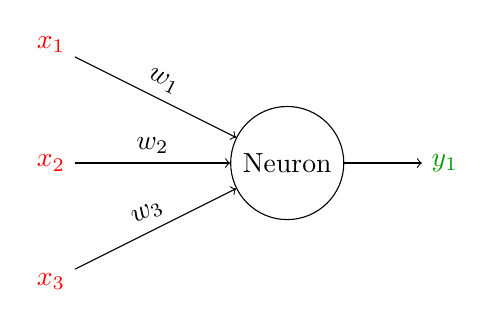
\begin{tikzpicture}
        \path (3,0) node [circle,draw](neuron){Neuron};
        \path[red] (0,1.5) node(x1){$x_1$} (0,0) node(x2){$x_2$} (0,-1.5) node(x3){$x_3$};
        \path[black!40!green] (5,0) node(y1){$y_1$};
        \draw[->] (x1) -- node[above,sloped]{$w_1$} (neuron);
        \draw[->] (x2) -- node[above,sloped]{$w_2$} (neuron);
        \draw[->] (x3) -- node[above,sloped]{$w_3$} (neuron);
        \draw[->] (neuron) -- (y1);


    \end{tikzpicture}
    \caption{ein Perzeptron}

\end{figure}

\subsubsection{Backpropagation}
\subsubsection{Feedforward Neural Network}
\subsubsection{Deep Learning}
Laengliche Neuronale Netze
\subsubsection{Universal Approximation Theorem}
Neural Network kann alles erlernen

\subsection{Autoencoder und Convolutional NN}
\subsubsection{Convolutional Neural Networks}
Conv2D, MaxPooling2D, UpSampling2D
\subsubsection{Autoencoder}
\subsubsection{Variational Autoencoder?}
\subsubsection{Detangled Autoencoder?}


\end{document}

%%% Local Variables:
%%% mode: latex
%%% TeX-master: "../main"
%%% End:
